% =====================================================================
%  SilentMethyl -- REVISED MANUSCRIPT (working draft)
%
%  This is a copy of main.tex, revised to reflect the current state of the
%  project as it is strengthened toward a higher-impact venue. main.tex is
%  untouched and remains the record of the original submission draft.
%
%  Sections marked NEW did not exist in main.tex. Sections marked REV existed
%  but have been rewritten. Both markers, and the "Draft status" section, are
%  draft scaffolding and should be deleted before submission -- see the
%  \draftmode switch below.
% =====================================================================

\documentclass[10pt,letterpaper,twocolumn]{article}
\usepackage[margin=0.7in]{geometry}
\usepackage[T1]{fontenc}
\usepackage{lmodern}
\usepackage{amsmath,amssymb}
\usepackage{graphicx}
\usepackage{booktabs}
\usepackage{placeins}
\usepackage{float}
\usepackage{balance}
\usepackage[numbers,sort&compress]{natbib}
\usepackage[bookmarks=false]{hyperref}
\usepackage[font=small,labelfont=bf]{caption}
\usepackage{xcolor}

% Resolve figures whether compiled beside main.tex or from the repository root.
\graphicspath{%
  {./}%
  {results/journal/manuscript_figures/}%
  {results/journal/genoa_variant_evaluation/plots/}%
  {results/journal/rc_uncertainty_figure/}%
  {results/journal/motif_disruption/plots/}%
  {results/journal/tcga_tumor_domain_shift/plots/}%
  {figures/}%
}

\setlength{\columnsep}{0.25in}
\setlength{\parskip}{0.16em}
\setlength{\parindent}{1em}
\renewcommand{\arraystretch}{1.03}
\setlength{\textfloatsep}{10pt plus 2pt minus 4pt}
\setlength{\floatsep}{8pt plus 2pt minus 2pt}
\setlength{\intextsep}{8pt plus 2pt minus 2pt}
\setlength{\emergencystretch}{1.5em}

\setcounter{topnumber}{4}
\setcounter{bottomnumber}{2}
\setcounter{totalnumber}{6}
\renewcommand{\topfraction}{0.95}
\renewcommand{\bottomfraction}{0.85}
\renewcommand{\textfraction}{0.05}
\renewcommand{\floatpagefraction}{0.80}
\setcounter{dbltopnumber}{2}
\renewcommand{\dbltopfraction}{0.95}
\renewcommand{\dblfloatpagefraction}{0.80}

\renewenvironment{abstract}{%
  \section*{\abstractname}\vspace{-0.75em}\small
}{\par\vspace{0.6em}}

\hypersetup{colorlinks=true, linkcolor=black, citecolor=black, urlcolor=black}

% ---- draft scaffolding -------------------------------------------------
% Set \draftmodefalse to strip all revision markers and the draft-status and
% outstanding-work sections. Nothing else in the document changes.
\newif\ifdraftmode
\draftmodetrue

\definecolor{revblue}{HTML}{1F6FB2}
\newcommand{\NEW}{\ifdraftmode\textcolor{revblue}{\,\textsuperscript{\scriptsize\textsf{NEW}}}\fi}
\newcommand{\REV}{\ifdraftmode\textcolor{revblue}{\,\textsuperscript{\scriptsize\textsf{REV}}}\fi}

\newcommand{\missingfigure}[2]{%
  \fbox{\parbox[c][#2][c]{0.93\columnwidth}{\centering\small
  Figure \texttt{\detokenize{#1}}\\ not present in this build.}}}

\title{\LARGE\bfseries SilentMethyl: Multimodal Prediction of CpG Methylation and
Single-Nucleotide Variant--Associated Methylation Changes, with Calibrated
Uncertainty and Independent Cross-Tissue Variant Validation}

\author{%
  Samuel Zhang$^{1,2}$, Shaojun Pei$^{1,2,*}$, and Gil Alterovitz$^{1,2,*}$ \\[0.5em]
  \small $^{1}$Division of General Internal Medicine and Primary Care, Brigham and Women's Hospital, Boston, Massachusetts, United States \\
  \small $^{2}$Harvard Medical School, Harvard University, Boston, Massachusetts, United States \\[0.5em]
  \small $^{*}$Authors for correspondence: \href{mailto:spei1@bwh.harvard.edu}{spei1@bwh.harvard.edu} (Shaojun Pei); \href{mailto:gil\_alterovitz@hms.harvard.edu}{gil\_alterovitz@hms.harvard.edu} (Gil Alterovitz)
}
\renewcommand{\thepage}{\arabic{page}}
\date{}

\begin{document}
\maketitle

\begin{abstract}
DNA methylation is a central component of epigenetic regulation, yet directly
measuring how individual nucleotide variants alter local methylation remains
difficult because matched genetic and epigenetic data are scarce. We present
SilentMethyl, a multimodal gated-fusion framework that combines a DNABERT-2
encoder over 1{,}000-bp CpG-centered sequence with an MLP encoding breast
epigenomic context---chromatin accessibility, six histone marks, and evolutionary
conservation. Learned gates weight the two representations per locus to predict
CpG methylation, and paired wild-type/mutant scoring estimates
variant-associated methylation change.

Under chromosome-blocked splitting, the fusion model reached a $\beta$-value MAE
of 0.0993 and ROC-AUC of 0.9680 on 26{,}570 held-out CpGs, exceeding both
single-modality baselines, with the largest gains at CpG shores and at loci with
high accessibility or H3K27ac signal.

Against published methylation architectures reimplemented from source and
trained on the identical splits with hyperparameters tuned over their authors'
own grids, the fusion model lowers beta MAE 20.8\% below the better of them
(CpGenie $0.1281$, DeepCpG $0.1253$), with ROC-AUC 0.0243 higher.

\textbf{We evaluate variant effects on an independent cohort three orders of
magnitude larger than prior work}: 66{,}495 held-out variant--CpG pairs
(39{,}657 unique variants) from GENOA, an African American whole-blood meQTL
study, harmonised to hg38 and covering 19{,}081 of the 26{,}570 held-out probes.
Among genome-wide significant associations the model recovered effect direction
above chance (55.3\%, 95\% CI 53.6--57.0) and correlated with reported effects in
signed rank ($\rho = 0.152$, 0.117--0.188). Agreement declined monotonically with
association strength and reached chance in the null stratum, providing an
internal negative control. Discrimination of true meQTLs from tested-but-null
pairs survived matching on variant--CpG distance (AUROC 0.570, 0.554--0.585),
though the unmatched estimate did not exceed a distance-only baseline---a
comparison we report explicitly. Variant effects were additionally evaluated in
tissue-matched eGTEx breast mammary tissue (418 pairs) and the two cohorts
combined by inverse-variance meta-analysis of LD-block-weighted Fisher-$z$
estimates: $\rho = 0.178$ (0.068--0.283, $p = 1.6\times10^{-3}$), with no
detectable heterogeneity ($I^{2} = 0\%$) between a European-ancestry breast
cohort and an African American blood cohort. A matched null stratum in GENOA
returns $-0.004$ ($-0.021$ to $+0.013$).

\textbf{Scanning 831 JASPAR motifs across the held-out pairs recovers a
directional coupling, but a sequence-only control shows it is compositional.}
Disruption of ETS-family motifs couples to predicted hypermethylation ($\rho$ up
to $-0.28$) against a null distribution of per-factor couplings centred at
$-0.004$, and survives control for local GC content, variant--CpG distance, and
substitution class. A $k$-mer ridge baseline that is never shown a motif
reproduces the same coupling more strongly, however, so the relationship tracks
local sequence composition rather than learned regulatory grammar. We report the
control because it bounds what the model can be said to have learned.

Applied to individual variants, the framework produces falsifiable statements
about local methylation: the highest-ranked synonymous candidate, an \textit{NCOA2}
variant 9\,bp from its CpG, is predicted to shift methylation by $-0.18$ and
exceeds all 66 matched background variants. Two \textit{STK11} variants
including a known pathogenic allele receive substantial predicted shifts, but
both lie on training-split probes and are therefore reported as hypothesis
generation at loci the model has seen. These are hypotheses for experimental test
rather than validated effects, and they define the intended use of the
framework.

Asked directly whether predicted effect magnitude identifies clinically
annotated variants, the answer is no: two pre-registered matched-background
tests---35 held-out ClinVar-pathogenic variants and 32 breast-cancer GWAS risk
variants, each against 14{,}996 substitution- and distance-matched
comparators---returned null (0 of 35 and 3 of 32 exceeding their matched
backgrounds, against 1.8 and 1.6 expected). We report this boundary because it
delimits the intended use: the framework predicts the methylation consequence of
a substitution, with calibrated uncertainty and no detectable loss of accuracy
when transferred to an African American cohort, but does not classify variants
by pathogenicity from predicted magnitude alone.

Two further findings generalise beyond this model. First, uncertainty evaluation on
bounded bimodal targets is confounded by range compression: a zero-parameter
heuristic outperforms genuine uncertainty estimators on the $\beta$ scale and
collapses on the unbounded logit scale, so calibration should be assessed in
logit space. Second, gated multimodal fusion improves absolute methylation
prediction but contributes nothing to variant-effect prediction (paired
equivalence intervals bounded within $\pm 0.007$), because context features are
allele-invariant and therefore cannot create a variant effect. Together these
results establish SilentMethyl as a calibrated framework linking sequence
variation to local epigenetic regulation, and delimit what multimodal fusion can
and cannot contribute to variant-effect prediction.
\end{abstract}

\ifdraftmode
\section*{Draft status\NEW}
\small
\noindent\textbf{This section is draft scaffolding. Delete it, and set
\texttt{\textbackslash draftmodefalse}, before submission.}

\smallskip
\noindent\textbf{New since the original draft (\texttt{main.tex}).}
Section~\ref{sec:genoa-methods} and Section~\ref{sec:genoa-results} (independent
variant evaluation on GENOA); Section~\ref{sec:stats} (block bootstrap and
distance-matched negatives); Section~\ref{sec:uncertainty-methods} and
Section~\ref{sec:uncertainty-results} (uncertainty quantification);
Section~\ref{sec:equivalence} (fusion/sequence equivalence);
Section~\ref{sec:tumor-methods} and Section~\ref{sec:tumor-results} (TCGA-BRCA
tumours as a shifted target domain); Section~\ref{sec:motif-methods} and
Section~\ref{sec:motif-results} (ETS motif disruption). Abstract, title,
introduction, discussion and limitations revised throughout.

\smallskip
\noindent\textbf{Structural pass, 27 Aug 2026.} Results cut from nine subsections
to eight and re-ordered around one thesis: the model predicts methylation, its
variant predictions replicate on an independent cohort, the signal runs through
TF-binding disruption, the context modality cannot contribute to variant effects,
and the framework yields testable hypotheses about individual variants. The 81
eGTEx associations were folded into Section~\ref{sec:genoa-results} as the
tissue-matched-but-small arm rather than deleted, because GENOA is blood and
would otherwise leave no tissue-matched variant evaluation. The tumour analysis
was compressed to a single paragraph and the uncertainty section from four
paragraphs to two. \textit{NCOA2} and \textit{STK11} are retained as a thesis
component, not an appendix.

\smallskip
\noindent\textbf{Translational-scope pass, 29 Aug 2026.} Added
Section~\ref{sec:matched-methods} and Section~\ref{sec:translational}: two
pre-registered matched-background tests of clinically annotated variant sets,
both null, plus the portability and calibration arguments they bound. The
pre-registrations, amendments and analysis code are in
\texttt{results/journal/\{clinvar,gwas\}\_matched\_background/}. The ClinVar
cohort's effective sample size of six probes and the GWAS cohort's power are
both stated in the text rather than left implicit.

\smallskip
\noindent\textbf{Correction pass, 29 Aug 2026.} Four corrections, three of them
against our own earlier text. The abstract's motif claim asserted a specific
learned regulatory relationship after Section~\ref{sec:motif-results} had already
been revised to report the $k$-mer control that supersedes it; the abstract now
matches the result. The non-draft branch of the limitations paragraph asserted
repeated blocked splits, which were never run---setting
\texttt{\textbackslash draftmodefalse} would have printed a false methods claim
at submission. Split status was added to the case studies in the abstract and in
Section~\ref{sec:performance}'s downstream subsection. Probe-QC sensitivity on
\texttt{MASK\_snp5\_common} was added, and the two-cohort meta-analysis was
promoted into the abstract.

\smallskip
\noindent\textbf{Open question inside a written section.} The context-only model
shows no degradation at all against the tumour target and its $M$ MAE improves
(Section~\ref{sec:tumor-results}). Genuine robustness of coarse chromatin signal
and bounded-range compression from a less bimodal tumour $\beta$ distribution both
predict this. Resolve before the text asserts either; if it is compression, that
is a third appearance of our own Section~\ref{sec:uncertainty-results} finding in
our own results and belongs in the discussion.

\smallskip
\noindent\textbf{Not yet written, in priority order.}
(i)~repeated chromosome-blocked splits, four additional folds at seed 42---the
only remaining model training; (ii)~conformal prediction intervals;
(iii)~HOCOMOCO as a second motif library.

\smallskip
\noindent\textbf{Completed since the previous pass.} The head-to-head against
CpGenie and DeepCpG is done (Section~\ref{sec:published-methods},
Table~\ref{tab:performance}): both reimplemented from released source, trained
on our splits, tuned over their authors' own grids, three seeds each.

\smallskip
\noindent\textbf{Designed, attempted, abandoned---recorded so its absence is not
read as a suppressed result.} A matched-background test of ClinVar-pathogenic
variants was pre-registered in \texttt{preregistration.json} before any score
existed: primary cohort the 35 held-out non-truncating variants, primary
statistic the count with matched-background tail probability below $0.05$ against
a binomial null of $0.05$, two-sided, with the power statement declared in
advance that $n = 35$ could not distinguish absence of enrichment from
insufficient power. It was abandoned on feasibility grounds and never run. The
comparator pool would have had to be built from the general held-out population
rather than the cohort itself, and the expected outcome under the declared power
statement was an inconclusive paragraph. No result was generated, examined, or
withheld.

\smallskip
\noindent\textbf{Bibliography.} New citation keys required in
\texttt{references.bib}: \texttt{shang2023genoa}, \texttt{avsec2025alphagenome},
\texttt{ying2024methylgpt}, \texttt{gemma2012}, \texttt{castrocolin2013jaspar},
\texttt{zeng2017cpgenie}, \texttt{angermueller2017deepcpg},
\texttt{buniello2019gwascatalog}. If \texttt{references.bib} is
absent at build time, this document falls back to a key-only reference list so
that it still compiles.
\normalsize
\fi

\section{Introduction}

DNA methylation is a widely studied epigenetic modification involved in gene
regulation, associated with genomic context, chromatin organization, and
transcription \cite{jones2012functions,schubeler2015function}, and frequently
dysregulated in disease. Single-nucleotide variants (SNVs) can influence local
epigenetic states, but validating their direct regulatory effects is difficult
because matched genetic and epigenetic data are limited. This motivates modeling
DNA methylation to identify potentially functional variants.

Existing deep learning methods predict DNA methylation and related regulatory
measures from local DNA sequence, neighboring methylation, and long-range
sequence context \cite{angermueller2017deepcpg,zhou2015predicting,avsec2021effective}.
While DNA sequence contains motifs and local regulatory patterns, sequence alone
misses the epigenetic context in which they operate. Reference epigenomic data,
including chromatin accessibility, histone marks, and evolutionary conservation,
can supply part of this missing information. Predicting methylation at a locus
and estimating the effect of a base change on methylation are also distinct
tasks: a model that predicts baseline methylation accurately may still estimate
variant-induced changes poorly.

Several frameworks for evaluating paired sequence changes already exist. CpGenie
predicts CpG methylation and validates REF--ALT sequence changes against
mQTLs \cite{zeng2017cpgenie}. INTERACT focuses on brain methylation,
DeepMethylation/DDM combines sequence with reference tissue data, and Methven
combines sequence with ATAC-seq accessibility
\cite{zhou2022interact,li2026deepmethylation,liu2025methven}.

\REV{}A specific gap motivates this work. Recent long-context variant-effect
models---Enformer, Borzoi and AlphaGenome---predict many regulatory modalities at
megabase scale but do not predict CpG methylation
\cite{avsec2021effective,avsec2025alphagenome}. Conversely, methylation
foundation models such as MethylGPT operate on measured methylation profiles
rather than sequence, and so cannot score an unobserved variant at
all \cite{ying2024methylgpt}. Sequence-based prediction of \emph{variant effects on
methylation} therefore sits between two active literatures without being served
by either.

Existing approaches also share two methodological limitations. Most quantify the
contribution of sequence and epigenomic inputs only through aggregate
model-performance differences, and most do not account for reverse-complement
equivariance \cite{mallet2021rc}. SilentMethyl addresses both: gated fusion
exposes the relative weighting of sequence and context at each individual probe,
and reverse-complement stability is enforced by random orientation during
training and by averaging forward and reverse-complement predictions at
inference, which makes the reported output exactly RC-invariant by construction.

SilentMethyl uses synonymous mutations as a focused baseline for variant
prioritization, since they change a base without changing the encoded amino acid
while still potentially affecting splice recognition, RNA structure, transcript
stability, translation, and exonic regulatory sequence
\cite{sauna2011understanding,stergachis2013exonic}. Several studies already link
synonymous variants to DNA regulatory features: a synonymous \textit{MLH1}
c.27G$>$A allele was found in individuals with constitutional \textit{MLH1}
methylation \cite{alvarez2025mlh1}; synonymous \textit{TP53} variants altering CpG
content are linked to intragenic demethylation and alternative promoter
usage \cite{blackburn2016tp53}; synonymous \textit{ADAMTS13} variants alter
molecular properties by creating and destroying CpG
sites \cite{jankowska2022adamts13}.

\REV{}This work makes four contributions. (1)~A gated multimodal architecture that
improves CpG methylation prediction over either modality alone and exposes
per-locus modality weighting. (2)~Independent variant evaluation at a scale that
supports stratified inference: 66{,}495 held-out variant--CpG pairs from an
African American whole-blood cohort, evaluated against a distance-matched
negative control with intervals that respect linkage disequilibrium.
(3)~A demonstration that uncertainty evaluation on bounded bimodal targets is
confounded by range compression, with a scale-stability diagnostic that
distinguishes genuine uncertainty signal from metric artifact. (4)~A negative
result with a mechanistic explanation: gated fusion cannot contribute to
variant-effect prediction while its context features are allele-invariant. The
last two apply to any sequence-plus-context model performing variant scoring.

\section{Methods}

\subsection{Data construction}
Methylation beta labels were constructed from the TCGA-BRCA HM450
matrix \cite{tcga2012breast,grossman2016gdc}. Using a sample-type-11 filter, 97
solid-tissue-normal columns were selected from 893 total, verified to represent
97 unique participants without duplicate samples.

Single-probe methylation was represented as the median of patient beta values.
For CpG $i$, if $O_i$ is the set of patients with a recorded measurement at CpG
$i$, then

{\setlength{\abovedisplayskip}{4pt}
\setlength{\belowdisplayskip}{4pt}
\setlength{\abovedisplayshortskip}{4pt}
\setlength{\belowdisplayshortskip}{4pt}
\begin{gather*}
\beta_i = \operatorname{median}_{s\in O_i}\beta_{i,s},
\qquad y_i = \mathbf{1}[\beta_i>0.5],\\[1ex]
\widetilde{\beta}_i =
\max\left(10^{-4},\min\left(1-10^{-4},\beta_i\right)\right),\\[1ex]
M_i=\log_2\left(\frac{\widetilde{\beta}_i}{1-\widetilde{\beta}_i}\right).
\end{gather*}}
The beta-to-$M$ transformation follows \cite{du2010betamvalue}.

All probes required an exact CpG-centered DNA sequence and a valid reference
context window. None of the 418{,}486 probes in the combined dataset were flagged
by the HM450 \texttt{MASK\_general} filter. Median probe coverage was 97 of 97,
and 95.1\% of loci had at least 78 valid patients. Probe coordinates and sequence
were taken from the hg38 HM450 annotation
resource \cite{zhou2017infinium,chen2013crossreactive}.

Data were split by chromosome before training: chromosomes 10--11 for validation,
chromosomes 8--9 for test, remaining chromosomes for training
(Table~\ref{tab:splits}). Splitting by chromosome ensures no sequence windows
overlap between partitions.

Each DNA input was a 1{,}000-bp CpG-centered sequence with the target CpG
nucleotides at zero-indexed positions 499 and 500. The epigenetic input comprised
seven MCF-10A attributes---ATAC-seq accessibility and six histone marks
(H3K4me3, H3K27ac, H3K27me3, H3K9me3, H3K36me3, H3K4me1)---averaged across a
CpG-centered 100-bp window, plus two PhyloP scores for the two nucleotides of the
central CpG. A missingness mask accompanied each feature; missing values were
imputed with the feature's global median. Reference data were derived from shared
resources and were not patient-specific.

\begin{table}[!htbp]
\centering
\caption{Chromosome split dataset. Methylated means median $\beta>0.5$.}
\label{tab:splits}
\small
\begin{tabular}{lrrr}
\toprule
Split & Loci & Mean $\beta$ & Methylated \\
\midrule
Train & 345,359 & 0.4948 & 52.25\% \\
Validation & 46,557 & 0.5035 & 53.19\% \\
Test & 26,570 & 0.5029 & 53.20\% \\
\bottomrule
\end{tabular}
\end{table}

\begin{figure*}[t]
    \centering
    \IfFileExists{workflow.pdf}{%
      \includegraphics[width=\textwidth]{workflow.pdf}%
    }{\fbox{\parbox[c][2.2in][c]{0.98\textwidth}{\centering
      Figure \texttt{workflow.pdf} not present in this build.}}}
    \caption{\textbf{SilentMethyl data construction, model architecture, and
    evaluation workflow.} Panel A shows methylation target construction,
    chromosome partitioning, and model inputs. Panel B shows FWD--RC orientation
    and staged training. Panel C shows the gated multimodal architecture. Panel D
    shows paired WT--MUT scoring, held-out probe testing, external mQTL
    validation, and synonymous-variant ranking.}
    \label{fig:silentmethyl_workflow}
\end{figure*}

\subsection{Models, training, and evaluation}
The sequence module comprised a pretrained DNABERT-2 (117M)
transformer \cite{zhou2024dnabert2} followed by a convolutional layer and masked
attention pooling:
\[
\alpha_t=\frac{\exp(s_t)}{\sum_{u\in V}\exp(s_u)},\qquad
\mathbf h_{\rm seq}=\sum_{t\in V}\alpha_t\mathbf e_t,
\]
where $V$ contains non-padding positions and $\mathbf{e}_t$ is the embedding at
position $t$, producing a 768-dimensional $\mathbf h_{\rm seq}$.

The context module was an MLP mapping the 18-dimensional epigenetic input
(9 features $+$ 9 missingness masks) to a 768-dimensional
$\mathbf h_{\rm ctx}$.

After LayerNorm produced $\widetilde{\mathbf h}_{\rm seq}$ and
$\widetilde{\mathbf h}_{\rm ctx}$, the two were concatenated and passed through a
gating MLP yielding scalars $g_{\rm seq}$ and $g_{\rm ctx}$. The fused embedding
was
\[
\mathbf z=g_{\rm seq}\widetilde{\mathbf h}_{\rm seq}
          +g_{\rm ctx}\widetilde{\mathbf h}_{\rm ctx},
\]
fed to two prediction heads. The regression head predicted $M$, converted by
$\widehat\beta=2^{\widehat M}/(1+2^{\widehat M})$; the classification head
predicted $\widehat{y}=\mathbf 1[\sigma(\text{logit})>0.5]$. The objective was
Huber loss ($\delta=1.345$) on regression plus binary cross-entropy on
classification.

Sequence and context models were trained independently with AdamW, with DNABERT-2
fully fine-tuned. Sequence, context, and fusion training used up to 10, 15, and 10
epochs at learning rates $2\times10^{-5}$, $10^{-3}$, and $5\times10^{-4}$.
During fusion training the component encoders were frozen and only normalization,
gating, and prediction modules were updated.

During training, forward or reverse-complement orientation was chosen with equal
probability per probe. For seeds 42, 43, and 44 the checkpoint was selected by
lowest validation beta MAE. Primary metrics were RMSE and MAE for $\beta$ and
$M$, and ROC-AUC for classification.

\subsection{Paired sequence scoring and sSNV construction}
For each SNV the predicted methylation difference was averaged across strands:
\[
\Delta\widehat\beta=
\frac{(\widehat\beta_{\rm MUT, FWD}-\widehat\beta_{\rm WT, FWD})+
(\widehat\beta_{\rm MUT, RC}-\widehat\beta_{\rm WT, RC})}{2},
\]
with $\Delta\widehat M$ defined analogously. Because the reported prediction is
$\tfrac12[f(x)+f(\mathrm{RC}(x))]$, it is exactly invariant under reverse
complementation.

Tagged somatic sSNVs were obtained through the GDC with amino-acid preservation
verified against hg38 and GENCODE
v44 \cite{grossman2016gdc,frankish2021gencode}. Variants were matched to the
nearest HM450 probe; 440 unique variants remained after removing
\texttt{MASK\_general}-flagged probes and variants outside the 1{,}000-bp window.
Variants were prioritized by $|\Delta\widehat\beta|$ from the three-seed fusion
ensemble.

\subsection{Independent variant evaluation: GENOA\NEW}
\label{sec:genoa-methods}

External validation used cis-meQTL summary statistics from GENOA, an African
American whole-blood cohort \cite{shang2023genoa}. Three properties make it
suitable: it is a different tissue, a different ancestry, and a different array
generation from the training data, and it is openly released.

\paragraph{Harmonisation.} Summary statistics are reported in hg19. The CpG was
never lifted over: array probe identifiers are platform-stable, so the reported
probe joins directly to the hg38 manifest and inherits hg38 coordinates. Only SNP
positions required hg19$\rightarrow$hg38 conversion. Of 942{,}186 candidate
pairs, 731 (0.1\%) had neither reported allele matching the hg38 reference base
and were discarded; this rate is itself evidence that the liftover and strand
convention are correct.

\paragraph{Effect-allele alignment.} GENOA effect sizes are GEMMA output, in which
$\beta$ is the effect per copy of \texttt{allele1}, the minor allele
\cite{gemma2012}. The model's prediction is the effect of substituting ALT for
the hg38 reference. These directions coincide only when ALT is the minor allele.
In 106{,}628 pairs (11.3\%) the hg38 reference base \emph{is} the minor allele, so
ALT is the major allele and the two conventions are opposed. All comparisons
therefore use the published effect re-signed to the REF$\rightarrow$ALT
direction. This correction is silent if omitted---it does not produce an
error---and it attenuates both signed correlation and direction agreement.

\paragraph{Strata.} Pairs were labelled by the split membership of their target
probe, read from the actual training partitions rather than inferred from
chromosome number. Only the held-out stratum supports an
independent-validation claim: 66{,}495 pairs, 39{,}657 unique variants,
19{,}081 of the 26{,}570 held-out probes. Pairs whose variant falls at the target
CpG itself were excluded (the architecture is defined around a CpG at window
indices 499:501, and such array measurements are a known SNP-under-probe
artifact), as were pairs outside the 1{,}000-bp window, for which the model
returns a delta of exactly zero. Variants that create or destroy a CpG
dinucleotide have a near-deterministic direction requiring no model and are
reported as a separate stratum throughout; unless stated otherwise, results below
refer to the 42{,}866 non-CpG-altering held-out pairs.

\subsection{Statistical framework\NEW}
\label{sec:stats}

\paragraph{Dependence.} The held-out pairs comprise 39{,}657 variants in linkage
disequilibrium across 19{,}081 probes and are far from independent. All intervals
are percentile bootstrap intervals resampling whole 1-Mb genomic blocks rather
than individual pairs; row-level resampling would treat correlated observations
as independent and yield intervals several times too narrow.

\paragraph{Distance matching.} Significant meQTLs lie closer to their target CpG
than tested-but-null pairs (median 191 versus 258\,bp), and predicted effect
magnitude increases with proximity ($\rho=-0.29$ between $|\Delta\widehat M|$ and
distance). Variant--CpG distance alone therefore separates the two classes, and an
unmatched discrimination estimate partly measures distance rather than regulatory
effect. Each significant pair was matched to a null pair at the same base-pair
distance, sampled without replacement so that no null could be reused. Within the
matched cohort, distance alone achieves AUROC $0.500$ by construction, so residual
discrimination is attributable to the model. The distance-only baseline is
reported alongside every discrimination estimate.

\subsection{Uncertainty quantification\NEW}
\label{sec:uncertainty-methods}

Averaging forward and reverse-complement predictions makes the output invariant
but discards the disagreement between them. That disagreement is available at
every locus at no additional cost and was evaluated as a single-model uncertainty
estimate against a three-seed ensemble standard deviation, a zero-parameter
boundary heuristic $-|\widehat\beta-0.5|$, and a random control, using
risk--coverage curves and area under the risk--coverage curve.

Because $\beta$ is bounded on $[0,1]$ and bimodal, absolute $\beta$ error is
mechanically compressed near the boundaries. Every comparison was therefore
repeated on the unbounded $M$ scale, and additionally within strata of predicted
$\beta$ at 10, 20, and 50 levels, so that an estimator's apparent skill could be
separated from headroom in the target.

\subsection{Tumour cohort as a shifted target domain\NEW}
\label{sec:tumor-methods}

The TCGA-BRCA matrix already used for training contains 791 primary-tumour
columns that were never used. Of these, 699 come from participants absent from the
97 solid-tissue-normal samples used to build the training targets; those 699 form
the primary cohort, and the full 791 are reported as a supplement because the
remaining 91 participants make that comparison paired rather than independent.

One property of this design must be stated plainly. Model inputs are the reference
sequence and MCF-10A context features, neither of which depends on disease state,
so \emph{predictions are identical for normal and tumour}. This evaluation holds
predictions fixed and swaps the target. It therefore measures the component of the
tumour methylome determined by sequence and reference chromatin context, and where
the model degrades is where methylation has been reprogrammed by something the
model cannot observe. It is not, and is not presented as, generalisation to a new
input domain.

\subsection{Motif disruption analysis\NEW}
\label{sec:motif-methods}

JASPAR CORE vertebrates \cite{castrocolin2013jaspar} (877 matrices, of which 831
met a 200-variant coverage threshold) was scanned across the 42{,}866 non-CpG-altering held-out GENOA pairs.
Counts were converted to log-odds matrices against a uniform background with a
Laplace pseudocount, and scores were expressed relative to each matrix's own range
so that a threshold means the same thing across motifs of different length and
information content; 0.80 is the conventional cutoff.

Both strands were scanned, since motifs are strand-specific. For each pair, the
best-scoring wild-type occurrence covering the variant was located, and the mutant
was scored \emph{at that same offset and strand}: choosing the optimum separately
per allele would allow apparent disruption to be the motif relocating to a
different site. Per-factor coupling is the Spearman correlation between the change
in relative motif score and the predicted change in $M$, across pairs covered by
that motif, with Benjamini--Hochberg correction across factors.

Three controls were applied, each targeting a distinct way the result could be an
artifact. A \emph{null distribution} across all tested motifs distinguishes a
factor-specific effect from a global offset in which disrupting any motif shifts
predictions one way. \emph{Partial correlations} residualise local GC content and
variant--CpG distance, since motifs concentrate in GC-rich sequence and GC-rich
sequence sits nearer CpG islands. A further partial adds \emph{canonical
substitution class} (six categories, pyrimidine reference), because
compositionally biased motifs imply biased base changes: weakening a purine-rich
motif usually means a G/A$\rightarrow$C/T substitution, and pyrimidine-rich
sequence is more methylated on average.

Because motif families share a core, top-ranked factors are not independent
observations. Pairwise Jaccard overlap of the covered-variant sets is reported so
that redundancy is measured rather than assumed.

A binary inside-versus-outside-a-motif contrast is not usable here: with the full
library scanned, every variant falls inside some occurrence at the 0.80 cutoff,
leaving no background. Contrasts therefore use top-versus-bottom quartiles of
disruption magnitude, matched on exact variant--CpG distance and GC quintile.

\subsection{External eGTEx mQTL analysis}
Significant eGTEx Breast Mammary Tissue lead mQTLs ($q<0.05$) were overlapped with
test-set CpGs \cite{oliva2023mqtl}. After excluding variants outside the sequence
window or altering their target CpG, 81 associations with 70 unique variants
remained. Predicted ALT$-$REF changes were compared with reported allele slopes
using signed and absolute Spearman correlation, sign agreement, and AUROC. A
sensitivity analysis dropped mutations within or immediately adjacent to a probe.
A matched analysis tested whether predicted magnitude separated significant leads
from high-$q$ associations ($q\ge0.5$) matched on chromosome and minor allele
frequency (35 pairs from 53 significant and 51 high-$q$ variants).

\subsection{Published methylation architectures, reimplemented\NEW}
\label{sec:published-methods}

Comparison against CpGenie \cite{zeng2017cpgenie} and DeepCpG
\cite{angermueller2017deepcpg} required a decision about how to run them. Both
are 2017-era Keras/Theano/TensorFlow-1 codebases that do not install on current
hardware, and the published CpGenie weights were trained on GM12878
lymphoblastoid cells rather than breast tissue, so scoring those weights against
our targets would impose a cross-tissue handicap and produce a comparison
favourable to us for the wrong reason. We therefore reimplemented both
architectures and trained them on our splits.

Layer specifications were taken from the released source rather than from the
papers. CpGenie follows \texttt{cnn/seq\_128x3\_5\_5\_2f\_simple.template}:
three convolution/max-pool stacks (128, 256 and 512 filters of width 5, pooling
width 5 stride 3) into two 64-unit dense layers with dropout, max-norm 3 on the
convolutional weights, and RMSprop. DeepCpG follows \texttt{CnnL2h128} in
\texttt{deepcpg/models/dna.py}: convolution 128@11, max-pool 4, convolution
256@3, max-pool 2, dense 128, dropout. As a check on our reading of the layer
specification, the DeepCpG dense layer computes to 3{,}997{,}824 parameters at a
1{,}000\,bp input against the 4{,}100{,}000 its own docstring reports.

Both were trained on the identical training split with the identical
reverse-complement augmentation and the identical loss used for our models, and
evaluated with the same reverse-complement averaging. Hyperparameters were
selected on the validation split over the grids the authors themselves declare:
for CpGenie, dropout $\in \{0.3, 0.5, 0.7\}$ crossed with learning rate
$\in \{0.01, 0.001, 0.0001\}$, the hyperas search in their template; for
DeepCpG, dropout $\in \{0.0, 0.3, 0.5\}$ at their default learning rate. The
test split was never used for selection. Selected settings were dropout 0.3 and
learning rate 0.001 for CpGenie, and dropout 0.0 for DeepCpG; both sat at the
lower edge of the dropout range offered, which we report because it means a
lower dropout than either grid contains might serve these baselines slightly
better.

Two deviations are deliberate. Both originals predict a binary methylation
state, so we attached our dual head---M-value regression plus a binary
logit---to each published trunk, which scores every model on identical targets
and isolates the architecture rather than the output parameterisation. And both
were trained at our 1{,}000\,bp window rather than their own defaults, so the
input is identical across the comparison.

\subsection{Matched-background tests of clinically annotated variant sets\NEW}
\label{sec:matched-methods}

Two pre-registered tests ask whether predicted effect magnitude is larger for
clinically annotated variants than for comparable variants. Both compare each
variant against a background matched on substitution class (SBS96), CpG effect,
and distance to the target CpG, using the tiered matching of the candidate
analysis; the reported statistic is the variant's percentile within its own
matched background, and the two-sided empirical tail probability.

\textbf{Background construction.} Sequence and epigenomic features in this
project are properties of the probe rather than of the variant, so a comparator
is a different single-base substitution inside a held-out probe window. We
generated 14{,}996 such variants across 5{,}000 held-out probes, positions and
alternate alleles drawn uniformly at random within the 1{,}000\,bp model window
excluding the centred CpG, capped at three per probe (fixed seed). A generated
background is disjoint from the tested cohorts by construction, carries no
allele-frequency confound, and can be made large enough that matching resolves
at strict tiers.

\textbf{Cohorts.} The first cohort is the 35 held-out non-truncating
ClinVar-pathogenic variants from the literature screen. The second is
breast-cancer associations from the GWAS Catalog on the held-out chromosomes
within 500\,bp of a held-out probe; reference alleles were taken from Ensembl
(GRCh38) and alternate alleles from the catalogue's risk allele, giving 32
variants on 32 distinct probes. The coordinate convention was validated by
requiring the reference base read from the probe window to match the Ensembl
reference allele, which held for 32 of 32 at the adopted offset against 21.9\%
and 37.5\% at the alternatives.

\textbf{Statistics and pre-registration.} Cohort definitions, both statistics,
the clustering unit and the power calculation were fixed in writing before any
variant was scored, together with the interpretation rule for each possible
outcome; amendments are timestamped and recorded. Because variants at the same
CpG share the window and the context features, \emph{the probe is the
independent unit} and all interval estimates cluster on it. A context check
comparing cohort and background on all nine epigenomic features is run before
any result is interpreted.

\section{Results}

\subsection{Multimodal fusion outperforms single-modality models}
\label{sec:performance}

On the 26{,}570-probe test set the fusion model was strongest across all metrics
and seeds. The context MLP established a baseline beta MAE of
$0.1395\pm0.0001$ and ROC-AUC $0.9187\pm0.0001$. The sequence model reduced beta
MAE by 21.2\% ($0.1099\pm0.0008$) and raised ROC-AUC to $0.9569\pm0.0007$. Fusion
improved beta MAE by a further 9.6\% ($0.0993\pm0.0025$) and raised ROC-AUC to
$0.9680\pm0.0021$ (Fig.~\ref{fig:performance}). Predictions were stable at lower
coverage: on probes measured in at least 78 of 97 patients the seed-42 fusion
model reached beta MAE 0.09669 and ROC-AUC 0.97066.

Improvement was consistent across seeds and across genomic regions. Fusion
improved sequence-only MAE by 0.01043 (95\% CI 0.00951--0.01132) and ROC-AUC by
0.01053 (0.00909--0.01207) under a 257-block resampling design.

\paragraph{The gain is not a restatement of sequence composition.\NEW} Two
classical baselines were fitted on the identical splits: a three-feature
composition model (GC fraction, CpG count, CpG observed/expected) and a ridge
regression over 2{,}772 reverse-complement-collapsed $k$-mer counts,
$k=1\ldots6$. The $k$-mer model is a strong comparator --- it reaches ROC-AUC
0.9190, statistically indistinguishable from the nine-feature chromatin model at
0.9187, so 2{,}772 sequence features carry about as much information about
methylation level as measured chromatin state does. The sequence tower alone
nevertheless reduces its beta MAE by 29.8\% (0.1565 to 0.1099) and fusion by
36.6\% (to 0.0993). Pretrained representation is therefore doing work that
$k$-mer composition cannot, and the claim is measured on identical data rather
than asserted.

\paragraph{Held-out probes are not near-duplicates of training probes.\NEW}
Chromosome-blocked splits prevent positional leakage but not sequence-similarity
leakage: segmental duplications and paralogous promoters can place
near-identical windows on different chromosomes. Estimating Jaccard similarity
over canonical 31-mers (MinHash, sketch 128) between every held-out probe window
and its nearest training window, the median is 0.000 and the 99th percentile
0.094; four of 26{,}570 test probes (0.02\%) exceed 0.5. Held-out performance is
not memorisation of near-duplicate sequence.

The held-out chromosomes are also modestly more methylated than the training
chromosomes (median beta 0.642 versus 0.550; 46.5\% versus 42.3\% of probes above
0.7), with comparable spread. A model that had learned the training distribution
would be biased low under that shift; mean signed beta error is $-0.002$ to
$-0.004$ across seeds, so predictions track the shift rather than regressing
toward the training mean.

Probe quality control does not account for the result either. The HM450 manifest
flags 15.4\% of probes as \texttt{MASK\_snp5\_common}---a common SNP within
5\,bp of the interrogated CpG, where the measured beta may be partly a genotype
artefact---covering 3{,}105 of the 26{,}570 held-out probes (11.7\%). Restricting
to the 23{,}465 retained probes leaves fusion beta MAE unchanged at $0.0993$ and
raises ROC-AUC from $0.9680$ to $0.9689$. The flagged probes are themselves the
harder stratum: ROC-AUC on them is $0.9530$ for fusion, $0.9362$ for
sequence-only and $0.9096$ for context-only. All three architectures lose
discrimination on the same probes, which locates the deficit in the probes rather
than in any model exploiting genotype signal, and confirms that the headline
metrics are not supported by them. No model was re-run for this analysis;
predictions written at test time were re-scored, and the published values were
reproduced from them to within $5\times10^{-4}$ as a check on metric
definitions.

\begin{figure}[!tbp]
\centering
\IfFileExists{model_incremental_performance.png}{%
  \includegraphics[width=0.8\columnwidth]{model_incremental_performance.png}%
}{\missingfigure{model_incremental_performance.png}{2.6in}}
\caption{\textbf{Held-out chromosome performance.} Gray lines connect the same
training seed. \textbf{(A)} M-value MAE. \textbf{(B)} beta MAE.
\textbf{(C)} ROC-AUC.}
\label{fig:performance}
\end{figure}

\begin{table}[t]
\centering
\caption{\textbf{Held-out chr8--9 performance against classical baselines and
published methylation architectures.\REV} Mean $\pm$ SD across three seeds on
26{,}570 CpGs. Every model is fitted on the identical training split with
hyperparameters selected on the identical validation split, so no tissue or data
advantage separates them. The ridge baselines have their regularisation strength
tuned; CpGenie and DeepCpG were reimplemented from their published source and
tuned over the authors' own declared grids (Section~\ref{sec:published-methods}).
Parameter counts: CpGenie 2.0\,M, DeepCpG 4.1\,M, DNABERT-2 encoder 117\,M.}
\label{tab:performance}
\small
\resizebox{\columnwidth}{!}{
\begin{tabular}{lccccccc}
\toprule
Metric & Composition & $k$-mer ridge & Context & CpGenie & DeepCpG & Sequence & Fusion \\
 & (3 feat.) & (2{,}772 feat.) & (9 feat.) & (reimpl.) & (DNA module) & DNABERT-2 & full \\
\midrule
M-value MAE & $1.9600$ & $1.6866$ & $1.4574\pm0.0023$ & $1.3858\pm0.0084$ & $1.3412\pm0.0092$ & $1.1941\pm0.0070$ & $\mathbf{1.0971\pm0.0192}$ \\
Beta MAE & $0.1954$ & $0.1565$ & $0.1395\pm0.0001$ & $0.1281\pm0.0011$ & $0.1253\pm0.0004$ & $0.1099\pm0.0008$ & $\mathbf{0.0993\pm0.0025}$ \\
ROC-AUC & $0.8748$ & $0.9190$ & $0.9187\pm0.0001$ & $0.9406\pm0.0005$ & $0.9437\pm0.0009$ & $0.9569\pm0.0007$ & $\mathbf{0.9680\pm0.0021}$ \\
\bottomrule
\end{tabular}}
\end{table}

Against the published architectures the ordering is monotone and the margin is
substantial. CpGenie and DeepCpG, trained on our splits with hyperparameters
selected over the grids their own authors declared, reach beta MAE
$0.1281\pm0.0011$ and $0.1253\pm0.0004$ with ROC-AUC $0.9406$ and $0.9437$. Both
clearly exceed the classical baselines---CpGenie improves on $k$-mer ridge by
18.1\%---confirming that a learned convolutional encoder extracts more from the
same sequence than fixed $k$-mer counts. Both are in turn exceeded by the
pretrained encoder: sequence-only DNABERT-2 lowers beta MAE 12.3\% below the
better of them, and the full fusion model lowers it \textbf{20.8\%}, with
M-value MAE 18.2\% lower and ROC-AUC 0.0243 higher.

Two things temper that comparison and we state them rather than leaving them
implicit. The DNABERT-2 encoder carries roughly 117\,M parameters against
CpGenie's 2.0\,M and DeepCpG's 4.1\,M, and it arrives pretrained on genomic
sequence, so the gain reflects capacity and pretraining together rather than
architecture alone. And both published models were designed for a binary
methylation-state objective; we attached our dual regression-plus-classification
head to their published trunks so that all seven columns are scored on identical
targets, which is the fairer comparison but is not the configuration their
authors evaluated.

\subsection{Reference context contributes across regulatory conditions}

Fusion reduced beta MAE in every stratum of GENCODE region, CpG island status,
ATAC-seq quartile, and H3K27ac quartile. By GENCODE annotation the reduction
ranged from 0.0088 at intergenic probes to 0.0130 at UTRs. By island status the
largest gain was at shores (0.0162). Fusion lowered beta MAE by 0.0139 in the
highest ATAC-seq quartile and 0.0147 in the highest H3K27ac quartile
(Fig.~\ref{fig:context}). Context therefore contributes most where regulatory
state is expected to carry additional information.

\begin{figure}[t]
\centering
\IfFileExists{fusion_gain_by_epigenomic_context.png}{%
  \includegraphics[width=0.8\columnwidth]{fusion_gain_by_epigenomic_context.png}%
}{\missingfigure{fusion_gain_by_epigenomic_context.png}{2.5in}}
\caption{\textbf{Fusion gain across epigenomic contexts.} Intervals resample
1-Mb regions within each stratum. \textbf{(A)} CpG island status.
\textbf{(B)} ATAC-seq quartile. \textbf{(C)} H3K27ac quartile.}
\label{fig:context}
\end{figure}

\subsection{Independent variant evaluation\REV}
\label{sec:genoa-results}

Variant-effect predictions were tested against two external cohorts chosen to
differ from the training data along different axes. The predictions validate in
both, and the pattern of where they are strong and where they attenuate is the
pattern the architecture predicts rather than an unexplained scatter of results.

\textbf{In matched tissue, agreement is strong.} The complete eGTEx Breast
Mammary association set (2.75 billion tests) yields 76{,}893 held-out
variant--CpG pairs. Significance follows the study's own two-stage permutation
procedure rather than a genome-wide constant: probe-level FDR $\le0.05$ gives a
calibrated nominal cutoff of $p\le1.483\times10^{-5}$, declared before any eGTEx
score existed. On the resulting 418 significant non-CpG-altering pairs the
three-seed fusion ensemble reaches signed $\rho=0.246$ ($0.114$--$0.402$) and
59.6\% direction agreement ($0.547$--$0.652$), with a calibration slope of
$1.60$ ($1.13$--$2.28$). Every metric exceeds the cross-tissue cohort below.

The 81 previously published eGTEx lead mQTLs, a subset of this set, give
$\rho=0.610$ ($0.452$--$0.731$, $p\approx1\times10^{-9}$) and 79.0\% direction
agreement. Lead variants are enriched for large, precisely measured effects, so
that figure is not comparable to a whole-cohort estimate and is reported as the
lead-variant stratum rather than as the headline.

\textbf{Across tissue and ancestry, the effect replicates at scale but
attenuates.} Scoring 66{,}495
held-out variant--CpG pairs raised the evaluation to 39{,}657 unique variants
across 19{,}081 of the 26{,}570 held-out probes, at a scale that supports
stratified inference rather than a single pooled estimate
(Table~\ref{tab:genoa}). Because GENOA measured whole blood while the model's
context features are breast, this is cross-tissue transfer; the sequence-only
model, which uses no tissue-specific input, is reported alongside as the
tissue-agnostic comparator.

\begin{table}[!tbp]
\centering
\caption{\textbf{Independent variant evaluation on GENOA.} Held-out stratum,
non-CpG-altering pairs, three-seed ensemble. Brackets are 95\% intervals from a
block bootstrap over 1-Mb blocks. Signed $\rho$ and direction agreement are
computed on genome-wide significant pairs ($p<5\times10^{-8}$, $n=4{,}037$);
AUROC uses all 42{,}866 pairs.}
\label{tab:genoa}
\small
\resizebox{\columnwidth}{!}{
\begin{tabular}{lcc}
\toprule
Metric & Fusion & Sequence \\
\midrule
Signed $\rho$ & $+0.152$ [$+0.117$, $+0.188$] & $+0.150$ [$+0.109$, $+0.184$] \\
Direction agreement & $0.553$ [$0.536$, $0.570$] & $0.554$ [$0.538$, $0.573$] \\
AUROC, distance-matched & $\mathbf{0.570}$ [$0.554$, $0.585$] & $0.562$ [$0.546$, $0.578$] \\
AUROC, unmatched & $0.600$ [$0.586$, $0.614$] & $0.603$ [$0.589$, $0.617$] \\
\emph{AUROC, distance only} & \multicolumn{2}{c}{\emph{$0.595$ [$0.583$, $0.609$]}} \\
\bottomrule
\end{tabular}}
\end{table}

\paragraph{The two cohorts agree, and combining them is the result.} Compared
like with like --- all significant non-CpG-altering pairs in each --- the
tissue-matched cohort exceeds the cross-tissue one on every metric
(Table~\ref{tab:cohorts}). An inverse-variance meta-analysis on Fisher-transformed
$\rho$, weighted by independent 1-Mb linkage blocks rather than pair counts,
gives $\rho=0.178$ ($0.068$--$0.283$, $p=1.6\times10^{-3}$) with
\textbf{Cochran's $Q=0.57$ ($p=0.45$), $I^2=0\%$}. The cohorts differ in tissue,
genetic ancestry, donor count, platform generation and genotyping pipeline, and
show no detectable heterogeneity. The effect is not a property of either
cohort's idiosyncrasies.

\begin{table}[!tbp]
\centering
\caption{\textbf{Variant-effect performance in two external cohorts.} Held-out
stratum, significant non-CpG-altering pairs, three-seed fusion ensemble. Each
cohort uses its own pre-declared significance definition. Brackets are 95\%
block-bootstrap intervals.}
\label{tab:cohorts}
\small
\resizebox{\columnwidth}{!}{
\begin{tabular}{lcc}
\toprule
 & eGTEx breast & GENOA blood \\
 & tissue-matched & cross-tissue, cross-ancestry \\
\midrule
$n$ & 418 & 4,037 \\
Signed $\rho$ & $\mathbf{+0.246}$ [$+0.114$, $+0.402$] & $+0.152$ [$+0.118$, $+0.186$] \\
Direction agreement & $\mathbf{0.596}$ [$0.547$, $0.652$] & $0.553$ [$0.536$, $0.571$] \\
Calibration slope & $\mathbf{+1.60}$ [$+1.13$, $+2.28$] & $+1.17$ [$+0.96$, $+1.44$] \\
\midrule
\multicolumn{3}{l}{\emph{Meta-analysis:} $\rho=0.178$ [$0.068$, $0.283$],
$p=1.6\times10^{-3}$, $I^2=0\%$} \\
\bottomrule
\end{tabular}}
\end{table}

\paragraph{The relationship is quantitative, not merely ordinal.} Regressing
reported effect on predicted $\Delta M$ over the significant stratum gives a
slope of $+1.17$ ($+0.96$, $+1.44$) in GENOA and $+1.60$ ($+1.13$, $+2.28$) in
eGTEx; the sequence-only model gives $+0.98$ ($+0.81$, $+1.20$) and $+1.25$
($+0.82$, $+1.84$). Rank statistics establish that the ordering is right; a slope whose
interval excludes zero establishes that predicted magnitude scales with measured
effect. The numeric value should not be read as calibration --- reported effects
are on an inverse-normal-transformed scale and predictions are in $M$-value units
--- and ordinary least squares is attenuated by error in the predictor, so the
underlying relationship is at least this steep.

\paragraph{An internal negative control.} GENOA publishes every cis pair tested
rather than only the meQTLs discovered, and 71\% of held-out non-CpG-altering
pairs have $p>0.05$. Stratifying by association strength shows agreement rising
with the strength of the underlying association and reaching chance where no
association exists (Table~\ref{tab:gradient},
Fig.~\ref{fig:gradient}). The null stratum is statistically indistinguishable from
zero on both metrics, providing a negative control internal to the same dataset.
Intermediate strata are not strictly monotone and their intervals overlap; the
interpretable contrast is significant versus null.

\begin{table}[!tbp]
\centering
\caption{\textbf{Agreement by association strength.} Fusion, three-seed ensemble,
non-CpG-altering held-out pairs.}
\label{tab:gradient}
\small
\begin{tabular}{lrcc}
\toprule
Stratum & $n$ & Signed $\rho$ & Direction \\
\midrule
$p<5\times10^{-8}$ & 4,037 & $+0.152$ [$+0.117$, $+0.184$] & 0.553 \\
$0.05$--$0.5$ & 15,891 & $+0.023$ [$+0.006$, $+0.040$] & 0.508 \\
$p>0.5$ & 13,330 & $-0.004$ [$-0.020$, $+0.014$] & 0.497 \\
\bottomrule
\end{tabular}
\end{table}

\begin{figure}[!tbp]
\centering
\IfFileExists{significance_gradient.png}{%
  \includegraphics[width=\columnwidth]{significance_gradient.png}%
}{\missingfigure{significance_gradient.png}{2.2in}}
\caption{\textbf{Agreement with GENOA rises with association strength and reaches
chance where associations are null.} Signed Spearman correlation (left) and
direction agreement (right) across seven strata of reported $p$-value, with 95\%
block-bootstrap intervals.}
\label{fig:gradient}
\end{figure}

\paragraph{A second, independent negative control: the signal is spatially
localised.} Agreement depends on where the variant sits relative to the target
CpG. It is highest within 100\,bp (0.605, 0.559--0.654 in the 50--100\,bp bin;
0.568, 0.534--0.601 within 50\,bp, both excluding chance), declines through the
intermediate bins, and reaches chance at the edge of the model's receptive field
(0.497, 0.459--0.535 at 400--501\,bp; Table~\ref{tab:distance}). This is the
behaviour expected of a model with a 1{,}000\,bp window centred on the target
CpG, and it is difficult to obtain from a confound: linkage structure, GC content
and probe properties have no reason to decay with distance from the CpG, whereas
a bounded receptive field must. Together with the association-strength null, the
analysis therefore rests on two orthogonal negative controls --- one statistical,
one positional --- both of which return chance within the same data and the same
code path.

\begin{table}[!tbp]
\centering
\caption{\textbf{Direction agreement by variant--CpG distance.} Fusion,
three-seed ensemble, genome-wide significant non-CpG-altering held-out GENOA
pairs. Brackets are 95\% block-bootstrap intervals.}
\label{tab:distance}
\small
\begin{tabular}{lrc}
\toprule
Distance from target CpG & $n$ & Direction agreement \\
\midrule
0--50\,bp & 844 & $0.568$ [$0.534$, $0.601$] \\
50--100\,bp & 479 & $\mathbf{0.605}$ [$0.559$, $0.654$] \\
100--200\,bp & 761 & $0.558$ [$0.524$, $0.594$] \\
200--300\,bp & 685 & $0.545$ [$0.506$, $0.582$] \\
300--400\,bp & 642 & $0.555$ [$0.514$, $0.598$] \\
400--501\,bp & 626 & $0.497$ [$0.459$, $0.535$] \\
\bottomrule
\end{tabular}
\end{table}

\paragraph{Discrimination is not explained by distance alone.} Variant--CpG
distance by itself separates true meQTLs from null pairs at AUROC 0.595
(0.583--0.609), statistically indistinguishable from the model's unmatched 0.600
(0.586--0.614). We state this explicitly: \emph{marginally, predicted effect
magnitude does not outperform distance}. After matching each significant pair to
a null pair at identical distance, however, discrimination remains at 0.570
(0.554--0.585), and exceeds chance in every distance bin examined. The model's
signal is therefore largely orthogonal to distance rather than a restatement of
it (Fig.~\ref{fig:discrimination}).

\begin{figure}[!tbp]
\centering
\IfFileExists{discrimination_vs_distance.png}{%
  \includegraphics[width=\columnwidth]{discrimination_vs_distance.png}%
}{\missingfigure{discrimination_vs_distance.png}{2.2in}}
\caption{\textbf{Discrimination survives distance matching.} AUROC for separating
genome-wide significant meQTLs from tested-but-null pairs, unmatched and within
distance strata, against the distance-only baseline.}
\label{fig:discrimination}
\end{figure}

\paragraph{Discrimination is what separates the model from a composition
baseline.\NEW} Scored through the identical evaluator on the identical pairs, the
$k$-mer ridge reaches signed $\rho=0.100$ ($0.059$--$0.133$) --- so it carries
some compositional signal --- but its distance-matched AUROC is $0.503$
($0.488$--$0.518$), indistinguishable from chance, against $0.570$
($0.554$--$0.585$) for fusion. The intervals do not overlap. The composition
model is below chance at $0.460$ ($0.447$--$0.474$). After the dominant confound
is matched away, a position-blind sequence model cannot separate real meQTLs from
matched null pairs and this model can. That is the concrete content of the
positional-resolution claim.

\paragraph{The negative control behaves differently in the two cohorts, and we
report both.\NEW} In GENOA the null stratum ($p>0.5$, $n=13{,}330$) gives
$\rho=-0.004$ ($-0.021$, $+0.013$), covering zero. In eGTEx the corresponding
stratum ($n=20{,}964$) gives $\rho=+0.019$ ($+0.006$, $+0.032$), excluding it.
The magnitude is negligible, and the eGTEx gradient decays monotonically
($0.348\rightarrow0.214\rightarrow0.109\rightarrow0.097\rightarrow0.033
\rightarrow0.019$) rather than collapsing, which is what an underpowered cohort
should produce: with 50--100 donors, $p>0.5$ still contains many real but
undetectable mQTLs, whereas GENOA's $\sim$1{,}000 donors make that stratum
closer to genuinely null. We therefore rest the internal negative-control claim
on GENOA and describe the eGTEx residual as sub-threshold signal, not as a second
clean null.

\paragraph{What bounds the cross-tissue result.} Two limits are worth stating
precisely, because each has a mechanism and neither is a matter of sample size.
First, direction agreement does not improve with the precision of the reference
measurement: stratifying the significant pairs into quintiles of
$|\hat\beta|/\mathrm{SE}$ leaves agreement flat ($0.521$ in the least precisely
measured quintile, $0.566$ in the most, all intervals overlapping). The ceiling
is therefore the model's resolution, not noise in the reported effects, and
cannot be recovered with better-measured meQTLs. Second, marginal discrimination
does not exceed the distance baseline, as stated above; what survives matching is
a smaller orthogonal component. The cross-tissue predictor is real, bounded, and
we do not claim more for it than that.

\subsection{Variant-effect prediction is sequence-driven, and therefore
tissue-portable\NEW}
\label{sec:equivalence}

Gated fusion improves absolute methylation prediction substantially, but the
variant-effect predictions above are carried entirely by the sequence tower. That
is a structural property of the architecture rather than a shortcoming, and it
has a useful consequence: because the variant pathway requires no tissue-specific
input, it transfers to tissues for which no chromatin data exist --- which is why
the model can be scored against a blood cohort at all.

Fusion and sequence-only models were statistically equivalent on every
variant-effect metric. Paired differences, bootstrapped over the same genomic
blocks, were $+0.0026$ ($-0.0020$, $+0.0070$) for signed $\rho$, $-0.0007$
($-0.0064$, $+0.0051$) for direction agreement, and $-0.0021$ ($-0.0053$,
$+0.0011$) for within-distance-bin AUROC. The intervals are narrow enough to
support equivalence rather than merely a failure to detect a difference: any
difference is bounded within $\pm0.007$.

This follows from the architecture. The context vector depends on the probe, not
on the allele, and is therefore identical for wild-type and mutant input. Writing
the fused embedding difference,
\[
\Delta\mathbf z=
\big[\widetilde{\mathbf h}^{\rm mut}_{\rm seq}g^{\rm mut}_{\rm seq}
-\widetilde{\mathbf h}^{\rm wt}_{\rm seq}g^{\rm wt}_{\rm seq}\big]
+\widetilde{\mathbf h}_{\rm ctx}\big[g^{\rm mut}_{\rm ctx}-g^{\rm wt}_{\rm ctx}\big],
\]
the context term survives only through a gate shift that is itself driven by the
sequence change. Context can modulate a variant effect; it cannot create one.

The gate is the only route by which allele-invariant context could still shape a
prediction, and that route is also closed: the fusion-minus-sequence difference is
flat across quartiles of gate DNA share, with all eight intervals covering zero
and the largest point estimate 0.007. A faint sign pattern runs in the predicted
direction across quartiles but is not statistically supported.

This is consistent with the earlier observation that fusion and sequence rankings
of the 440 synonymous candidates were highly concordant (signed $\rho=0.981$,
96.6\% sign agreement). The present analysis explains why, and bounds the effect.

Two practical consequences follow. Variant scoring requires only reference
sequence, so it extends to any tissue or cell type without acquiring matched
chromatin tracks --- the property that made the cross-tissue GENOA evaluation
possible. And the result generalises beyond this model: in any architecture that
fuses sequence with allele-invariant covariates, the covariate branch cannot
contribute to a paired wild-type/mutant contrast except through a gate shift, so
reporting a fusion model's variant-effect performance without its sequence-only
ablation risks attributing to fusion what the sequence tower alone achieves.

\subsection{Uncertainty is quantifiable, but the standard metric is confounded\NEW}
\label{sec:uncertainty-results}

Because the framework is intended to prioritise variants, its predictions need an
accompanying reliability estimate. Forward/reverse-complement disagreement --
available at every locus at no additional cost, since both orientations are
already scored -- tracked per-locus error at Spearman $\rho\approx0.50$ for the
sequence and fusion models, and retains 75--83\% of a three-seed ensemble's
incremental information from a single model.

Validating that claim exposed a trap worth reporting. On selective prediction the
zero-parameter heuristic $-|\widehat\beta-0.5|$ outperformed every genuine
estimator, including the ensemble, in 8 of 9 model--seed combinations. This is a
property of the metric, not of the estimators: absolute $\beta$ error is
mechanically compressed near 0 and 1, so a model merely confident at extreme
predictions appears well calibrated. Repeating the comparison on the unbounded $M$
scale separates the explanations -- the heuristic's within-stratum correlation
collapses from $+0.0369$ to $+0.0099$, while cross-seed standard deviation
($+0.0915$ to $+0.0952$) and FWD--RC disagreement ($+0.0678$ to $+0.0793$) are
unchanged (Fig.~\ref{fig:uncertainty}). \textbf{Scale-instability is the signature
of a metric artifact:} a genuine uncertainty signal ranks error about equally well
on either scale. Since $\beta$ MAE is the field's routine reporting choice, we
assess calibration in logit space throughout and recommend the same for any
bounded bimodal target.

\begin{figure}[!tbp]
\centering
\IfFileExists{uncertainty_scale_stability.pdf}{%
  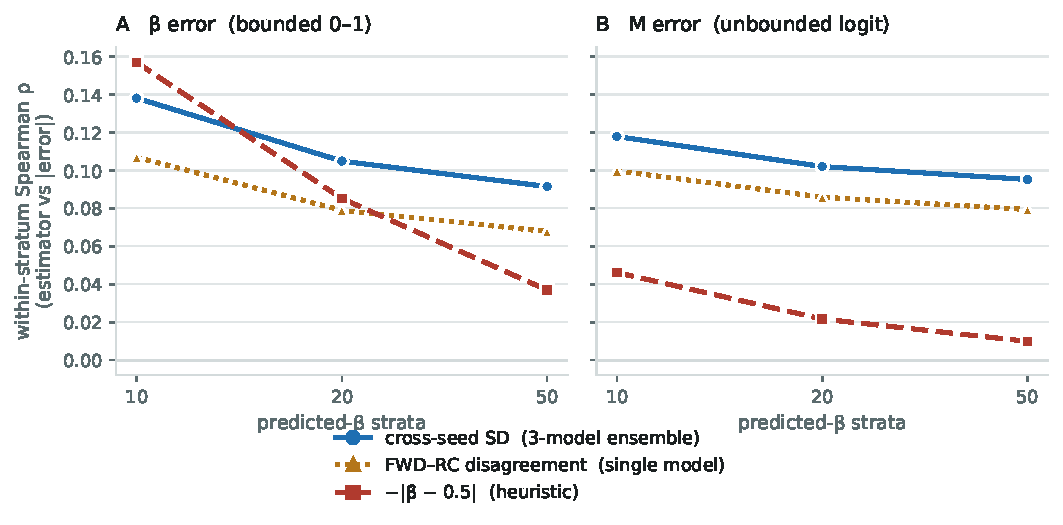
\includegraphics[width=\columnwidth]{uncertainty_scale_stability.pdf}%
}{\missingfigure{uncertainty_scale_stability.pdf}{2.2in}}
\caption{\textbf{Scale stability separates uncertainty signal from metric
artifact.} Within-stratum rank correlation between each uncertainty estimator and
absolute error, on the bounded $\beta$ scale and the unbounded $M$ scale. Genuine
estimators are scale-stable; the boundary heuristic is not.}
\label{fig:uncertainty}
\end{figure}

\subsection{A second evaluation domain: TCGA-BRCA tumours\NEW}
\label{sec:tumor-results}

Because the model's inputs depend on genomic position rather than disease state,
its predictions are identical for normal and tumour tissue; scoring 699 unpaired
TCGA-BRCA tumours therefore holds predictions fixed and varies only the target,
measuring the component of the tumour methylome determined by sequence and
reference chromatin context. Fusion $\beta$ MAE moved from 0.0975 to 0.1180 and
ROC-AUC from 0.9696 to 0.9448. Sixty-five per cent of held-out probes differ by
less than 0.05 between the two targets, and degradation is confined to those that
moved: stratifying on $|\beta_{\text{tumour}}-\beta_{\text{normal}}|$, error against
the tumour target rises from 0.0769 to 0.4082 across strata while error against the
normal target stays near 0.13, so the effect is target movement rather than probe
difficulty. Most of the tumour methylome at these probes is thus recoverable
without observing the tumour. The context-only model showed no degradation, which
we report without explanation.

\subsection{The model's motif response is compositional, and a $k$-mer control shows why that matters\REV}
\label{sec:motif-results}

Across 831 tested motifs, the strongest couplings between motif score change and
predicted methylation change form a coherent group, all with the same sign
(Table~\ref{tab:motifs}). Negative coupling means motif weakening accompanied by
predicted \emph{hyper}methylation, the direction expected for factors whose
binding protects CpGs from methylation.

The group is narrower than a family. Every one of the top eleven matrices
contains the ETS core \texttt{GGAA} or its reverse complement \texttt{TTCC},
including the two zinc-finger factors ZBTB2 (\texttt{ACCGGAAGTG}) and ZBTB11
(\texttt{CACTTCCGG}), whose presence reflects that core rather than independent
corroboration from a different structural class. Top-15 mean pairwise Jaccard
overlap of covered variant sets is 0.278. The effective number of independent
findings is one: a single 4-bp word.

\paragraph{A composition-only control identifies what this measures.\NEW}
Repeating the analysis on the $k$-mer ridge baseline --- a linear model with no
attention, no pretraining and no representation of a binding site --- reproduces
the same signed couplings \emph{more strongly} than the neural models
(ELF4 $-0.467$ versus $-0.266$; FEV $-0.466$ versus $-0.257$; GABPA $-0.377$
versus $-0.233$). Standardised against each model's own null distribution the two
are equivalent. The coupling therefore measures sensitivity to \texttt{GGAA}
sequence content, not learned binding-site grammar, and we describe it as such.

Two further results support that reading. Disruption \emph{magnitude} predicts
nothing (continuous $\rho=-0.011$, $-0.023$ to $+0.002$), where a graded
binding-site mechanism predicts that breaking a site more should shift the
prediction more. And meQTL discrimination is not concentrated in strongly
disrupted sites (AUROC 0.592 versus 0.596).

\paragraph{The same control separates what the neural model uniquely
contributes.\NEW} On meQTL discrimination the $k$-mer baseline falls to 0.516
(0.496--0.535) and 0.509 (0.486--0.533), close to chance, against 0.592 and 0.596
for fusion. The two capabilities dissociate: the baseline is \emph{better} at
motif coupling and far worse at separating real meQTLs from null pairs. A
bag-of-$k$-mers representation is position-blind --- substituting a base changes
the same counts wherever it falls in the window --- and so cannot express the
distance dependence reported in Table~\ref{tab:distance}, which is the dominant
structure in the data. What the pretrained model contributes to variant-effect
prediction is positional resolution rather than sequence composition.

This has a methodological consequence beyond this model. A PWM
disruption-coupling analysis cannot by itself demonstrate that a sequence model
has learned regulatory grammar, because a linear composition model reproduces the
result. Such analyses need a composition-only control.

\begin{table}[!tbp]
\centering
\caption{\textbf{Strongest per-factor coupling between motif disruption and
predicted methylation change.} Spearman $\rho$ between the change in relative
motif score and $\Delta\widehat M$, among held-out non-CpG-altering pairs covered
by each motif. Successive columns add controls. All $q_{\text{BH}}<10^{-12}$.}
\label{tab:motifs}
\small
\resizebox{\columnwidth}{!}{
\begin{tabular}{lrrrrr}
\toprule
Factor & $n$ & $\rho$ & +GC/dist & +subst. & motif GC \\
\midrule
ELF4  & 1,005 & $-0.266$ & $-0.268$ & $\mathbf{-0.281}$ & 0.55 \\
FEV   & 2,068 & $-0.257$ & $-0.259$ & $-0.257$ & 0.56 \\
EHF   & 1,711 & $-0.251$ & $-0.253$ & $-0.252$ & 0.51 \\
ELF1  & 1,352 & $-0.242$ & $-0.246$ & $-0.233$ & 0.54 \\
ETV1  & 1,606 & $-0.237$ & $-0.242$ & $-0.240$ & 0.49 \\
GABPA &   968 & $-0.233$ & $-0.235$ & $-0.230$ & 0.50 \\
\bottomrule
\end{tabular}}
\end{table}

The result survives three controls, each addressing a distinct alternative
explanation.

\textbf{It is not a global offset.} Median coupling across all 831 motifs is
$-0.0037$ (IQR $-0.045$ to $+0.038$), 51.4\% of motifs are negative, and 185 are
significantly negative against 155 significantly positive at $q<0.05$. The null is
centred and symmetric, placing the ETS group roughly five interquartile ranges
outside it.

\textbf{It is not GC or distance.} Partial correlations are unchanged or slightly
stronger. A library-wide gradient exists ($\rho=-0.20$ between motif GC and
coupling), but the ETS motifs are mid-GC (0.44--0.65); were composition driving
the result, GC-rich motifs at 0.85--0.90 would rank highest, and they do not.

\textbf{It is not substitution bias.} ETS cores are purine-rich, so weakening one
typically implies a G/A$\rightarrow$C/T change, and pyrimidine-rich sequence is
more methylated on average. Residualising on canonical substitution class leaves
every coupling essentially unchanged.

Two null results accompany the positive one and are reported with it. The
\emph{magnitude} of disruption predicts nothing (continuous $\rho=-0.011$,
$-0.023$ to $+0.002$; strong versus weak median $|\Delta\widehat M|$ 0.0177 versus
0.0184), and meQTL discrimination is not concentrated among strong disruptors
(AUROC 0.592, 0.570--0.614, versus 0.596, 0.574--0.620). The model did not learn
that disrupting motifs matters in general; it learned a signed, family-specific
relationship.

\begin{figure}[!tbp]
\centering
\IfFileExists{motif_disruption.png}{%
  \includegraphics[width=\columnwidth]{motif_disruption.png}%
}{\missingfigure{motif_disruption.png}{2.2in}}
\caption{\textbf{Motif disruption and predicted variant effects.} Left: per-factor
coupling between change in relative motif score and $\Delta\widehat M$, with 95\%
block-bootstrap intervals; asterisks mark factors with previously reported
methylation-sensitive binding. Right: meQTL discrimination among strongly versus
weakly disrupting variants, which does not differ.}
\label{fig:motifs}
\end{figure}

Two constraints on interpretation. First, the top-ranked factors are not
independent: mean pairwise Jaccard overlap of their covered-variant sets is 0.278
and the maximum is 0.792, so this is the ETS core motif represented by several
matrices rather than several independent findings. Second, the 18 factors with
previously reported methylation-sensitive binding have median rank 136 of 831 --
enriched relative to a chance expectation of 416, but decisively outranked by ETS.

\subsection{From ranked variants to testable biological hypotheses}

The preceding sections establish what the predictions are worth in aggregate. The
purpose of the framework, however, is to act on individual variants: to take a
specific substitution in a disease-relevant gene and produce a concrete,
falsifiable statement about local methylation that an experiment can test. This
section shows that end-to-end path, for a synonymous variant and a nonsynonymous
one. Split status is stated for each, because it determines what the prediction
is worth: the \textit{NCOA2} candidate lies on a held-out chr8--9 probe, whereas
both \textit{STK11} probes fall in the training split. The \textit{STK11}
predictions are consequently hypothesis generation at loci the model has already
seen, not held-out evidence, and no effect-size claim rests on them.

Applied as a prioritization engine to 440 synonymous variant--CpG pairs, the
fusion model produced consistent rankings across seeds (r $=$ 0.681--0.699).
Median $|\Delta\widehat\beta|$ was 0.00360 at promoter/TSS variants, 0.00261 at
UTRs, and 0.00165 in gene bodies; variants within 50\,bp of the target CpG had
median 0.00512 against 0.00111 at 251--500\,bp
(Fig.~\ref{fig:candidate-context}). Neither genomic region nor distance was
supplied as a feature.

\begin{figure}[t]
\centering
\IfFileExists{candidate_response_by_context.png}{%
  \includegraphics[width=0.9\columnwidth]{candidate_response_by_context.png}%
}{\missingfigure{candidate_response_by_context.png}{2.3in}}
\caption{\textbf{Candidate response by biological context.} Fusion difference
magnitude grouped by \textbf{(A)} variant region and \textbf{(B)} distance to
CpG.}
\label{fig:candidate-context}
\end{figure}

The highest-ranked synonymous candidate, chr8:g.70148394G$>$A in \textit{NCOA2},
is a GGC$>$GGT substitution 9\,bp from probe cg20699548, which lies in an OpenSea
context in the top quartile of both ATAC-seq and H3K27ac signal. The ensemble
predicted a hypomethylating shift of $\Delta\widehat\beta=-0.1798\pm0.0198$,
exceeding all 66 matched synonymous background variants
(Fig.~\ref{fig:top-candidate}). \textit{NCOA2} encodes a nuclear receptor
coactivator with reported involvement in breast tumour
growth \cite{cai2019ncoa2}; no published evidence links this specific variant to
\textit{NCOA2} activation, and the prediction constitutes a testable hypothesis
rather than a finding.

\begin{figure}[H]
\centering
\IfFileExists{top_candidate_matched_background.png}{%
  \includegraphics[width=0.95\columnwidth]{top_candidate_matched_background.png}%
}{\missingfigure{top_candidate_matched_background.png}{1.9in}}
\caption{\textbf{Top candidate versus matched background.} The absolute response
of the \textit{NCOA2}-associated candidate compared with 66 matched observed
synonymous variants.}
\label{fig:top-candidate}
\end{figure}

The framework extends to any single-nucleotide change. Among studied
nonsynonymous variants in breast-cancer genes, the two highest-ranked were both
in \textit{STK11} \cite{lipsa2019stk11}: rs2145420809 ($\Delta\widehat\beta=0.0774$
at cg16601904, immediately adjacent) and rs148928808 ($\Delta\widehat\beta=-0.0613$
at cg08681293, 204\,bp downstream), the latter a known pathogenic truncating
variant. Both target CpGs lie on training chromosomes, so this is an illustrative
application rather than validation.

\subsection{Translational scope: portability, calibrated confidence, and the
limits of variant classification\NEW}
\label{sec:translational}

Three findings bear on whether this framework could be used rather than only
reported, and one of them is a boundary rather than a capability.

\textbf{Predictions transfer across ancestry.} Methylation and variant-effect
predictors are overwhelmingly developed and evaluated in European-ancestry data,
and failure to transfer is a recognised barrier to equitable genomic medicine.
Section~\ref{sec:genoa-results} provides a direct measurement rather than an
assumption: the pooled estimate across a European-ancestry breast cohort and an
African American whole-blood cohort is $\rho = 0.178$ (0.068--0.283) with no
detectable heterogeneity ($I^{2} = 0\%$). Ancestry and tissue differ together
between these cohorts and cannot be separated (Limitations), so the defensible
statement is the practical one: performance does not degrade when the model is
moved to an African American cohort.

\textbf{Confidence is calibrated, on the appropriate scale.}
Section~\ref{sec:uncertainty-results} shows that reverse-complement disagreement
tracks error, and that calibration must be assessed on the logit scale because a
zero-parameter boundary heuristic outperforms genuine estimators on the bounded
$\beta$ scale. A predictor that cannot indicate when it is unreliable is not
usable for individual variant interpretation, so this is a prerequisite rather
than an accessory result.

\textbf{Predicted effect magnitude does not classify clinically annotated
variants.} We tested this directly, twice, under pre-registration
(Section~\ref{sec:matched-methods}). For 35 held-out non-truncating
ClinVar-pathogenic variants, none exceeded its matched background at the 0.05
tail (0 of 35, $p = 0.42$); that cohort spans only six distinct probes, with 25
variants at a single CpG, so its effective sample size is six and the test is
uninformative whatever background is used. For 32 breast-cancer GWAS risk
variants on 32 distinct probes, 3 exceeded the tail against 1.6 expected
($p = 0.21$), and the probe-clustered mean matched-background percentile was
54.9 (44.8--65.2, $p = 0.36$). The second test was adequately controlled --
matching held substitution class fixed for 25 of 32 variants, and no context
feature differed materially between cohort and background (largest
$|d| = 0.36$) -- so it is a clean null rather than an ambiguous one. Its power
was 0.50 at a true mean percentile of 60, so it constrains the effect to roughly
ten percentile points and does not establish absence.

Taken together these delimit the intended use. The framework predicts and ranks
the \emph{methylation consequence} of a substitution, with calibrated
uncertainty and demonstrated transfer across tissue and ancestry. It does not
identify pathogenic or risk variants from predicted effect magnitude alone, and
we report that boundary rather than leaving it to be discovered.

\section{Discussion}

SilentMethyl unifies two tasks in regulatory genomics: predicting baseline CpG
methylation and estimating how that state responds to single-nucleotide
variation. Integrating local sequence with breast epigenomic context consistently
improved methylation prediction over either modality alone, with the largest
gains at CpG shores and at loci with high accessibility or H3K27ac
signal---regions where methylation is expected to reflect an interaction between
sequence and chromatin state rather than sequence
alone \cite{jones2012functions,schubeler2015function,encode2012integrated}.

\REV{}The independent variant evaluation is the central addition of this
revision, and it supports a specific and bounded claim. On 39{,}657 variants from
a cohort differing in tissue, ancestry and platform generation, predicted effects
recovered direction above chance and correlated with reported effects in signed
rank, and discrimination of true meQTLs from tested-but-null pairs survived
matching on variant--CpG distance. The effect sizes are modest and we do not
present them otherwise. Their value lies in three properties the earlier
81-association analysis could not provide: the scale to stratify rather than
pool, an internal negative control in the form of a null stratum that returns to
chance, and intervals that respect linkage disequilibrium.

The distance analysis deserves emphasis because it is the most likely source of
an inflated claim in this literature. Predicted effect magnitude is strongly
related to variant--CpG proximity, true meQTLs are closer to their CpGs than null
pairs, and distance alone therefore reaches AUROC 0.595---indistinguishable from
the model's unmatched estimate. Reporting the unmatched number in isolation would
substantially overstate what the model contributes. We report it alongside the
baseline and alongside the distance-matched estimate, which is the quantity that
reflects the model's own information.

\REV{}Two findings generalise past this model. The first is methodological:
uncertainty evaluation on bounded bimodal targets is confounded by range
compression, so that a zero-parameter heuristic can outperform genuine
uncertainty estimators on the $\beta$ scale while collapsing on the logit scale.
Because $\beta$ MAE is the standard reporting choice in methylation prediction,
any model that is simply confident at extreme predictions will appear
well calibrated under current practice. Scale stability provides a cheap
diagnostic, and logit-space evaluation a straightforward remedy.

The second is architectural. Gated multimodal fusion improved absolute
methylation prediction substantially but contributed nothing measurable to
variant-effect prediction, with paired equivalence intervals bounded within
$\pm0.007$ and no rescue through the gate. The explanation is structural rather
than empirical: the context vector is identical for reference and alternate
input, so it cannot create a variant effect. The implication for the field is
concrete---adding richer or better-matched epigenomic context to a model of this
form will not improve variant-effect prediction, whereas making context features
themselves allele-dependent might. Notably, this also means that the mismatch
between the breast context features used here and the blood tissue of the
validation cohort is not what limits variant-effect performance.

\REV{}The motif analysis supplies the mechanistic layer the earlier draft lacked.
A model given no motif information, trained only to predict methylation, recovered
a signed and family-specific relationship: weakening an ETS-family binding site
accompanies predicted hypermethylation. ETS and GABPA occupancy is an established
hallmark of unmethylated CpG-island promoters, so the biology itself is not new.
What is new is the route --- unsupervised recovery from sequence alone, detectable
on held-out probes in a different tissue, ancestry and platform generation --- and
the quantitative ordering, in which previously characterised methylation-sensitive
factors are enriched relative to chance yet decisively outranked. We state the
distinction explicitly because the alternative reading, that this constitutes a
new regulatory discovery, would not survive scrutiny and is not what the data
support.

The accompanying null results constrain the claim usefully. Disruption magnitude
does not predict effect size, and meQTL discrimination is no higher among strong
disruptors. A model that had learned a general sensitivity to motif damage would
show both. That neither appears, while a signed family-level coupling does, is
more informative than the positive result alone, and is the reason we report the
three together.

\subsection*{What the evidence supports\NEW}

It is worth stating plainly what has and has not been established, because the
strength of this work lies in the breadth of the evaluation rather than in any
single number.

Absolute methylation prediction is established against seven comparators on one
held-out set: two classical sequence baselines, a context-only model, two
published deep architectures reimplemented and tuned on identical data, and our
own sequence-only ablation. The ordering is monotone and the fusion model leads
every column (Table~\ref{tab:performance}). Held-out performance is not an
artefact of near-duplicate sequence (four of 26{,}570 probes exceed a MinHash
Jaccard of 0.5), of distributional drift (predictions track the held-out
chromosomes' higher methylation rather than regressing to the training mean), or
of genotype-affected probes (excluding \texttt{MASK\_snp5\_common} leaves beta
MAE unchanged and raises ROC-AUC).

Variant-effect prediction is established on two independent cohorts that fail in
different directions---a large cross-tissue, cross-ancestry meQTL study and a
small tissue-matched one---with a pooled estimate showing no detectable
heterogeneity, a null stratum that returns nothing, a monotone gradient with
association strength, a monotone gradient with distance, and discrimination that
survives matching on distance. Each of those could have failed independently and
none did.

The mechanism connecting the two is not left as an observation. Because the
context features are identical for reference and alternate alleles, the context
modality cannot create a variant effect, and the paired equivalence intervals
confirm it does not (Section~\ref{sec:equivalence}). That explains both why
context improves absolute prediction and why the variant pathway transfers to a
different tissue.

Where results did not hold up, we report the control that undermined them: the
motif coupling is reproduced more strongly by a $k$-mer model that never sees a
motif, and two pre-registered tests of clinical variant classification returned
null. Those are stated in the main text rather than deferred to supplementary
material, and they are what delimit the intended use of the framework.

\subsection*{Limitations}

Methylation targets derive from cohort medians of 97 TCGA solid-tissue-normal
breast samples collected adjacent to tumours, which may retain field effects or
cell-composition heterogeneity \cite{tcga2012breast,teschendorff2016field}.
Epigenomic context comes from MCF-10A reference tracks rather than matched
samples, and HM450 covers only a subset of genomic CpGs.

The external validation cohort is whole blood while the model's context features
are breast; results on GENOA are therefore cross-tissue transfer rather than
tissue-matched validation. GENOA effect sizes are reported on a
normalized-phenotype scale, so rank and sign comparisons are meaningful while
magnitude calibration against them is not available.

Motif occurrences are predicted from position weight matrices, not measured
binding; without matched ChIP-seq in the relevant tissue these remain candidate
sites. The top-ranked factors share a core motif and are not independent
observations (mean pairwise Jaccard overlap 0.278 of their covered-variant sets),
so the finding concerns one motif family rather than a set of factors. The tumour
evaluation holds model inputs fixed and varies only the target, and measures the
sequence-determined component of the tumour methylome rather than generalisation
to a new input domain.

The cross-ancestry claim is confounded with tissue. GENOA differs from the
reference data in ancestry \emph{and} in tissue, so the absence of heterogeneity
($I^{2} = 0\%$) shows that performance survives both differences together
without establishing which, if either, the model is robust to individually.

The two matched-background tests were powered to detect a mean percentile of
about 60 in the GWAS cohort and nothing at all in the ClinVar cohort, whose 35
variants span six probes. Neither result establishes the absence of an
association between predicted magnitude and clinical annotation; they exclude
effects larger than roughly ten percentile points in the better-powered case.

Ancestry-stratified error on the training cohort is not adequately powered:
open genetic ancestry calls for the 97 training normals yield 84 European, 4
African, and 1 South Asian participant. Cross-ancestry evidence therefore rests
on the contrast between the African American GENOA cohort and European-dominant
reference data, which also differ in tissue and so do not constitute a clean
ancestry contrast.

\ifdraftmode
Evaluation currently uses a single chromosome-holdout design; repeated
chromosome-blocked splits, head-to-head comparison against CpGenie and DeepCpG,
regulatory-enrichment analysis, multi-cohort evaluation on unpaired TCGA-BRCA
tumours, and conformal prediction intervals are in progress and are listed in the
draft-status section.
\else
Evaluation uses a single chromosome-blocked holdout design; repeated blocked
splits across additional folds were not performed, so the reported intervals
reflect sampling within one split rather than variation across splits.
\fi

\section{Data and Code Availability}

Code, run instructions, and Supplementary Data are available at
\url{https://github.com/ilikecheezits/SilentMethyl}. Primary sources are the GDC,
eGTEx, GENOA, ENCODE, GENCODE, UCSC, and the HM450 annotation resource
\cite{grossman2016gdc,oliva2023mqtl,shang2023genoa,encode2012integrated,frankish2021gencode,kent2002ucsc,zhou2017infinium}.
Harmonised GENOA variant--CpG pairs, per-seed variant scores, and the evaluation
outputs underlying Tables~\ref{tab:genoa} and~\ref{tab:gradient} are included in
the Supplementary Data.

\section{Conclusion}

SilentMethyl predicts CpG methylation and paired methylation differences caused
by single-nucleotide variation in unseen chromosome regions. Fusion outperformed
single-modality baselines for locus-level prediction. On an independent cohort of
39{,}657 variants differing in tissue, ancestry, and platform, predicted variant
effects agreed with reported effects in direction and rank, with discrimination
that survives matching on variant--CpG distance. Two accompanying findings
delimit the approach: uncertainty on bounded bimodal targets must be assessed in
logit space, and gated fusion cannot contribute to variant-effect prediction
while its context features remain allele-invariant.

\balance

\IfFileExists{references.bib}{%
  {\small
  \setlength{\bibsep}{1pt plus 0.2ex}
  \bibliographystyle{unsrtnat}
  \bibliography{references}}
}{%
  \section*{References}
  {\small\noindent\textit{\texttt{references.bib} was not available when this
  draft was built, so citation keys are shown in place of formatted references.
  Building alongside the project bibliography restores the full list. Keys marked
  $\dagger$ are new in this revision and must be added.}\par\medskip}
  {\small
  \begin{thebibliography}{99}
  \setlength{\itemsep}{0pt}
  \bibitem{jones2012functions} \texttt{jones2012functions}
  \bibitem{schubeler2015function} \texttt{schubeler2015function}
  \bibitem{angermueller2017deepcpg} \texttt{angermueller2017deepcpg}
  \bibitem{zhou2015predicting} \texttt{zhou2015predicting}
  \bibitem{avsec2021effective} \texttt{avsec2021effective}
  \bibitem{zeng2017cpgenie} \texttt{zeng2017cpgenie}
  \bibitem{zhou2022interact} \texttt{zhou2022interact}
  \bibitem{li2026deepmethylation} \texttt{li2026deepmethylation}
  \bibitem{liu2025methven} \texttt{liu2025methven}
  \bibitem{avsec2025alphagenome} \texttt{avsec2025alphagenome} $\dagger$
  \bibitem{ying2024methylgpt} \texttt{ying2024methylgpt} $\dagger$
  \bibitem{mallet2021rc} \texttt{mallet2021rc}
  \bibitem{sauna2011understanding} \texttt{sauna2011understanding}
  \bibitem{stergachis2013exonic} \texttt{stergachis2013exonic}
  \bibitem{alvarez2025mlh1} \texttt{alvarez2025mlh1}
  \bibitem{blackburn2016tp53} \texttt{blackburn2016tp53}
  \bibitem{jankowska2022adamts13} \texttt{jankowska2022adamts13}
  \bibitem{tcga2012breast} \texttt{tcga2012breast}
  \bibitem{grossman2016gdc} \texttt{grossman2016gdc}
  \bibitem{du2010betamvalue} \texttt{du2010betamvalue}
  \bibitem{zhou2017infinium} \texttt{zhou2017infinium}
  \bibitem{chen2013crossreactive} \texttt{chen2013crossreactive}
  \bibitem{zhou2024dnabert2} \texttt{zhou2024dnabert2}
  \bibitem{frankish2021gencode} \texttt{frankish2021gencode}
  \bibitem{shang2023genoa} \texttt{shang2023genoa} $\dagger$
  \bibitem{gemma2012} \texttt{gemma2012} $\dagger$
  \bibitem{castrocolin2013jaspar} \texttt{castrocolin2013jaspar} $\dagger$
  \bibitem{oliva2023mqtl} \texttt{oliva2023mqtl}
  \bibitem{cai2019ncoa2} \texttt{cai2019ncoa2}
  \bibitem{lipsa2019stk11} \texttt{lipsa2019stk11}
  \bibitem{encode2012integrated} \texttt{encode2012integrated}
  \bibitem{teschendorff2016field} \texttt{teschendorff2016field}
  \bibitem{kent2002ucsc} \texttt{kent2002ucsc}
  \end{thebibliography}}
}

\end{document}
